\documentclass[]{article}
\usepackage{lmodern}
\usepackage{amssymb,amsmath}
\usepackage{ifxetex,ifluatex}
\usepackage{fixltx2e} % provides \textsubscript
\ifnum 0\ifxetex 1\fi\ifluatex 1\fi=0 % if pdftex
  \usepackage[T1]{fontenc}
  \usepackage[utf8]{inputenc}
\else % if luatex or xelatex
  \ifxetex
    \usepackage{mathspec}
  \else
    \usepackage{fontspec}
  \fi
  \defaultfontfeatures{Ligatures=TeX,Scale=MatchLowercase}
\fi
% use upquote if available, for straight quotes in verbatim environments
\IfFileExists{upquote.sty}{\usepackage{upquote}}{}
% use microtype if available
\IfFileExists{microtype.sty}{%
\usepackage{microtype}
\UseMicrotypeSet[protrusion]{basicmath} % disable protrusion for tt fonts
}{}
\usepackage[margin=1in]{geometry}
\usepackage{hyperref}
\hypersetup{unicode=true,
            pdftitle={Find-a-gene Project},
            pdfborder={0 0 0},
            breaklinks=true}
\urlstyle{same}  % don't use monospace font for urls
\usepackage{color}
\usepackage{fancyvrb}
\newcommand{\VerbBar}{|}
\newcommand{\VERB}{\Verb[commandchars=\\\{\}]}
\DefineVerbatimEnvironment{Highlighting}{Verbatim}{commandchars=\\\{\}}
% Add ',fontsize=\small' for more characters per line
\usepackage{framed}
\definecolor{shadecolor}{RGB}{248,248,248}
\newenvironment{Shaded}{\begin{snugshade}}{\end{snugshade}}
\newcommand{\KeywordTok}[1]{\textcolor[rgb]{0.13,0.29,0.53}{\textbf{#1}}}
\newcommand{\DataTypeTok}[1]{\textcolor[rgb]{0.13,0.29,0.53}{#1}}
\newcommand{\DecValTok}[1]{\textcolor[rgb]{0.00,0.00,0.81}{#1}}
\newcommand{\BaseNTok}[1]{\textcolor[rgb]{0.00,0.00,0.81}{#1}}
\newcommand{\FloatTok}[1]{\textcolor[rgb]{0.00,0.00,0.81}{#1}}
\newcommand{\ConstantTok}[1]{\textcolor[rgb]{0.00,0.00,0.00}{#1}}
\newcommand{\CharTok}[1]{\textcolor[rgb]{0.31,0.60,0.02}{#1}}
\newcommand{\SpecialCharTok}[1]{\textcolor[rgb]{0.00,0.00,0.00}{#1}}
\newcommand{\StringTok}[1]{\textcolor[rgb]{0.31,0.60,0.02}{#1}}
\newcommand{\VerbatimStringTok}[1]{\textcolor[rgb]{0.31,0.60,0.02}{#1}}
\newcommand{\SpecialStringTok}[1]{\textcolor[rgb]{0.31,0.60,0.02}{#1}}
\newcommand{\ImportTok}[1]{#1}
\newcommand{\CommentTok}[1]{\textcolor[rgb]{0.56,0.35,0.01}{\textit{#1}}}
\newcommand{\DocumentationTok}[1]{\textcolor[rgb]{0.56,0.35,0.01}{\textbf{\textit{#1}}}}
\newcommand{\AnnotationTok}[1]{\textcolor[rgb]{0.56,0.35,0.01}{\textbf{\textit{#1}}}}
\newcommand{\CommentVarTok}[1]{\textcolor[rgb]{0.56,0.35,0.01}{\textbf{\textit{#1}}}}
\newcommand{\OtherTok}[1]{\textcolor[rgb]{0.56,0.35,0.01}{#1}}
\newcommand{\FunctionTok}[1]{\textcolor[rgb]{0.00,0.00,0.00}{#1}}
\newcommand{\VariableTok}[1]{\textcolor[rgb]{0.00,0.00,0.00}{#1}}
\newcommand{\ControlFlowTok}[1]{\textcolor[rgb]{0.13,0.29,0.53}{\textbf{#1}}}
\newcommand{\OperatorTok}[1]{\textcolor[rgb]{0.81,0.36,0.00}{\textbf{#1}}}
\newcommand{\BuiltInTok}[1]{#1}
\newcommand{\ExtensionTok}[1]{#1}
\newcommand{\PreprocessorTok}[1]{\textcolor[rgb]{0.56,0.35,0.01}{\textit{#1}}}
\newcommand{\AttributeTok}[1]{\textcolor[rgb]{0.77,0.63,0.00}{#1}}
\newcommand{\RegionMarkerTok}[1]{#1}
\newcommand{\InformationTok}[1]{\textcolor[rgb]{0.56,0.35,0.01}{\textbf{\textit{#1}}}}
\newcommand{\WarningTok}[1]{\textcolor[rgb]{0.56,0.35,0.01}{\textbf{\textit{#1}}}}
\newcommand{\AlertTok}[1]{\textcolor[rgb]{0.94,0.16,0.16}{#1}}
\newcommand{\ErrorTok}[1]{\textcolor[rgb]{0.64,0.00,0.00}{\textbf{#1}}}
\newcommand{\NormalTok}[1]{#1}
\usepackage{graphicx,grffile}
\makeatletter
\def\maxwidth{\ifdim\Gin@nat@width>\linewidth\linewidth\else\Gin@nat@width\fi}
\def\maxheight{\ifdim\Gin@nat@height>\textheight\textheight\else\Gin@nat@height\fi}
\makeatother
% Scale images if necessary, so that they will not overflow the page
% margins by default, and it is still possible to overwrite the defaults
% using explicit options in \includegraphics[width, height, ...]{}
\setkeys{Gin}{width=\maxwidth,height=\maxheight,keepaspectratio}
\IfFileExists{parskip.sty}{%
\usepackage{parskip}
}{% else
\setlength{\parindent}{0pt}
\setlength{\parskip}{6pt plus 2pt minus 1pt}
}
\setlength{\emergencystretch}{3em}  % prevent overfull lines
\providecommand{\tightlist}{%
  \setlength{\itemsep}{0pt}\setlength{\parskip}{0pt}}
\setcounter{secnumdepth}{0}
% Redefines (sub)paragraphs to behave more like sections
\ifx\paragraph\undefined\else
\let\oldparagraph\paragraph
\renewcommand{\paragraph}[1]{\oldparagraph{#1}\mbox{}}
\fi
\ifx\subparagraph\undefined\else
\let\oldsubparagraph\subparagraph
\renewcommand{\subparagraph}[1]{\oldsubparagraph{#1}\mbox{}}
\fi

%%% Use protect on footnotes to avoid problems with footnotes in titles
\let\rmarkdownfootnote\footnote%
\def\footnote{\protect\rmarkdownfootnote}

%%% Change title format to be more compact
\usepackage{titling}

% Create subtitle command for use in maketitle
\newcommand{\subtitle}[1]{
  \posttitle{
    \begin{center}\large#1\end{center}
    }
}

\setlength{\droptitle}{-2em}

  \title{Find-a-gene Project}
    \pretitle{\vspace{\droptitle}\centering\huge}
  \posttitle{\par}
    \author{}
    \preauthor{}\postauthor{}
    \date{}
    \predate{}\postdate{}
  

\begin{document}
\maketitle

\subsection{Generating the identity heatmap of multiple sequence
alignment for MuSK
family.}\label{generating-the-identity-heatmap-of-multiple-sequence-alignment-for-musk-family.}

Calculating the identity matrix

\begin{Shaded}
\begin{Highlighting}[]
\KeywordTok{library}\NormalTok{(bio3d)}
\NormalTok{seq.aln <-}\StringTok{ }\KeywordTok{read.fasta}\NormalTok{(}\StringTok{"Seqalignment_MuSK.fasta"}\NormalTok{)}
\NormalTok{seq.ide <-}\StringTok{ }\KeywordTok{seqidentity}\NormalTok{(seq.aln)}
\end{Highlighting}
\end{Shaded}

Plot identity matrix in heatmap form

\begin{Shaded}
\begin{Highlighting}[]
\KeywordTok{heatmap}\NormalTok{(seq.ide, }\DataTypeTok{symm =} \OtherTok{TRUE}\NormalTok{, }\DataTypeTok{labRow =}\NormalTok{ seq.aln}\OperatorTok{$}\NormalTok{id, }\DataTypeTok{labCol =}\NormalTok{ seq.aln}\OperatorTok{$}\NormalTok{id, }\DataTypeTok{margins =} \KeywordTok{c}\NormalTok{(}\DecValTok{9}\NormalTok{,}\FloatTok{7.5}\NormalTok{))}
\end{Highlighting}
\end{Shaded}

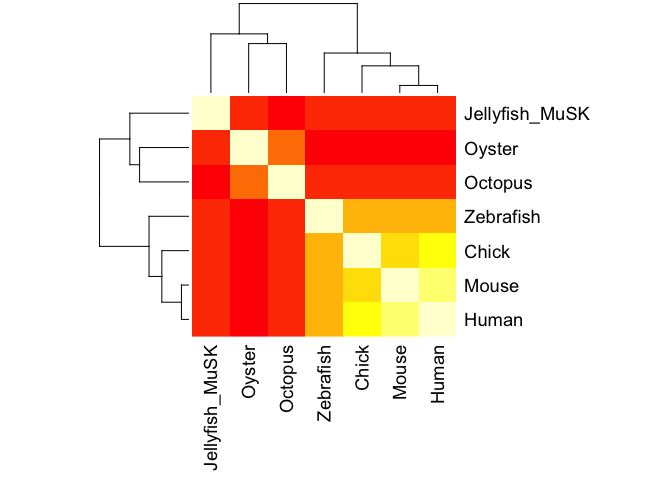
\includegraphics{Find_a_gene_Project_files/figure-latex/unnamed-chunk-2-1.pdf}

\subsection{Search the main protein structure database for the most
similar atomic resolution structures to your aligned
sequences.}\label{search-the-main-protein-structure-database-for-the-most-similar-atomic-resolution-structures-to-your-aligned-sequences.}

Generating consensus sequence from the alignment

\begin{Shaded}
\begin{Highlighting}[]
\NormalTok{seq.conss <-}\StringTok{ }\KeywordTok{consensus}\NormalTok{(seq.aln)}
\end{Highlighting}
\end{Shaded}

Since the consensus sequence might have a lot of gaps due to Jellyfish
MuSK is quite distant from some other organisms, human MuSK (the
row-wise maximum identity to other sequences used in alignment) will be
used to search for similar atomic resolution structures.

\begin{Shaded}
\begin{Highlighting}[]
\NormalTok{seq4pdb <-}\StringTok{ }\KeywordTok{read.fasta}\NormalTok{(}\StringTok{"data/Sequence_for_PDB_search.txt"}\NormalTok{)}
\NormalTok{pdbhits <-}\StringTok{ }\KeywordTok{blast.pdb}\NormalTok{(seq4pdb)}
\end{Highlighting}
\end{Shaded}

\begin{verbatim}
##  Searching ... please wait (updates every 5 seconds) RID = 8H50KTFP015 
##  ..............................................................
##  Reporting 100 hits
\end{verbatim}

Add annotation to the pdbhits result

\begin{Shaded}
\begin{Highlighting}[]
\NormalTok{pdbhits.anno <-}\StringTok{ }\KeywordTok{pdb.annotate}\NormalTok{(}\KeywordTok{substr}\NormalTok{(pdbhits}\OperatorTok{$}\NormalTok{hit.tbl}\OperatorTok{$}\NormalTok{pdb.id, }\DecValTok{1}\NormalTok{,}\DecValTok{4}\NormalTok{), }\DataTypeTok{anno.terms =} \KeywordTok{c}\NormalTok{(}\StringTok{"structureId"}\NormalTok{, }\StringTok{"experimentalTechnique"}\NormalTok{, }\StringTok{"resolution"}\NormalTok{, }\StringTok{"source"}\NormalTok{), }\DataTypeTok{unique =} \OtherTok{TRUE}\NormalTok{)}
\NormalTok{pdbhits.report <-}\StringTok{ }\KeywordTok{data.frame}\NormalTok{(pdbhits.anno, pdbhits}\OperatorTok{$}\NormalTok{hit.tbl}\OperatorTok{$}\NormalTok{evalue, pdbhits}\OperatorTok{$}\NormalTok{hit.tbl}\OperatorTok{$}\NormalTok{identity)}
\KeywordTok{colnames}\NormalTok{(pdbhits.report) <-}\StringTok{ }\KeywordTok{c}\NormalTok{(}\StringTok{"Id"}\NormalTok{, }\StringTok{"Technique"}\NormalTok{, }\StringTok{"Resolution"}\NormalTok{, }\StringTok{"Source"}\NormalTok{, }\StringTok{"Evalue"}\NormalTok{, }\StringTok{"Identity"}\NormalTok{)}
\KeywordTok{print.data.frame}\NormalTok{(pdbhits.report[}\DecValTok{1}\OperatorTok{:}\DecValTok{3}\NormalTok{,], }\DataTypeTok{row.names =} \OtherTok{FALSE}\NormalTok{)}
\end{Highlighting}
\end{Shaded}

\begin{verbatim}
##    Id         Technique Resolution            Source   Evalue Identity
##  1LUF X-RAY DIFFRACTION       2.05 Rattus norvegicus 3.69e-77   46.094
##  4YNE X-RAY DIFFRACTION       2.02      Homo sapiens 2.07e-75   44.672
##  5I8A X-RAY DIFFRACTION       2.33      Homo sapiens 2.31e-75   44.672
\end{verbatim}


\end{document}
